\begin{abstract}

Our analysis of the key-value activity generated by the ParSplice molecular
dynamics simulation demonstrates the need for more complex cache management
strategies. Baseline measurements show clear keyspace access patterns and hot
spots that offer significant opportunity for optimization. We use the Mantle
policy engine to dynamically explore a variety of techniques, ranging from
basic algorithms and heuristics to statistical models, calculus, and machine
learning. While Mantle was originally designed for distributed file systems, we
show how it effectively decomposes the problem into manageable policies for a
different domain and service (in this case, cache management).  Our exploration
of this space results in a two policy scheme that achieves 96\% efficiency
while using only 7.6\% of the memory resources required by the base case. 

\end{abstract}

\section{Introduction}

The fine-grained data annotation capabilities provided by key-value storage is
a natural match for many types of scientific simulation. Simulations relying on
a mesh-based decomposition of a physical region may result in millions or
billions of mesh cells. Each cell contains materials, pressures, temperatures
and other characteristics that are required to accurately simulate phenomena of
interest. In our target application, the
ParSplice~\cite{perez:jctc20150parsplice} molecular dynamics simulation, a
hierarchy of cache nodes and a single node key-value store are used to store
both observed minima across a molecule's equation of motion (EOM) and the
hundreds or thousands of partial trajectories calculated each second during a
parallel job. Unfortunately, if we scale the system the IO to the storage
hierarchy will quickly saturate both the storage and bandwidth capacity of a
single node. 

\begin{figure}[t]
  \noindent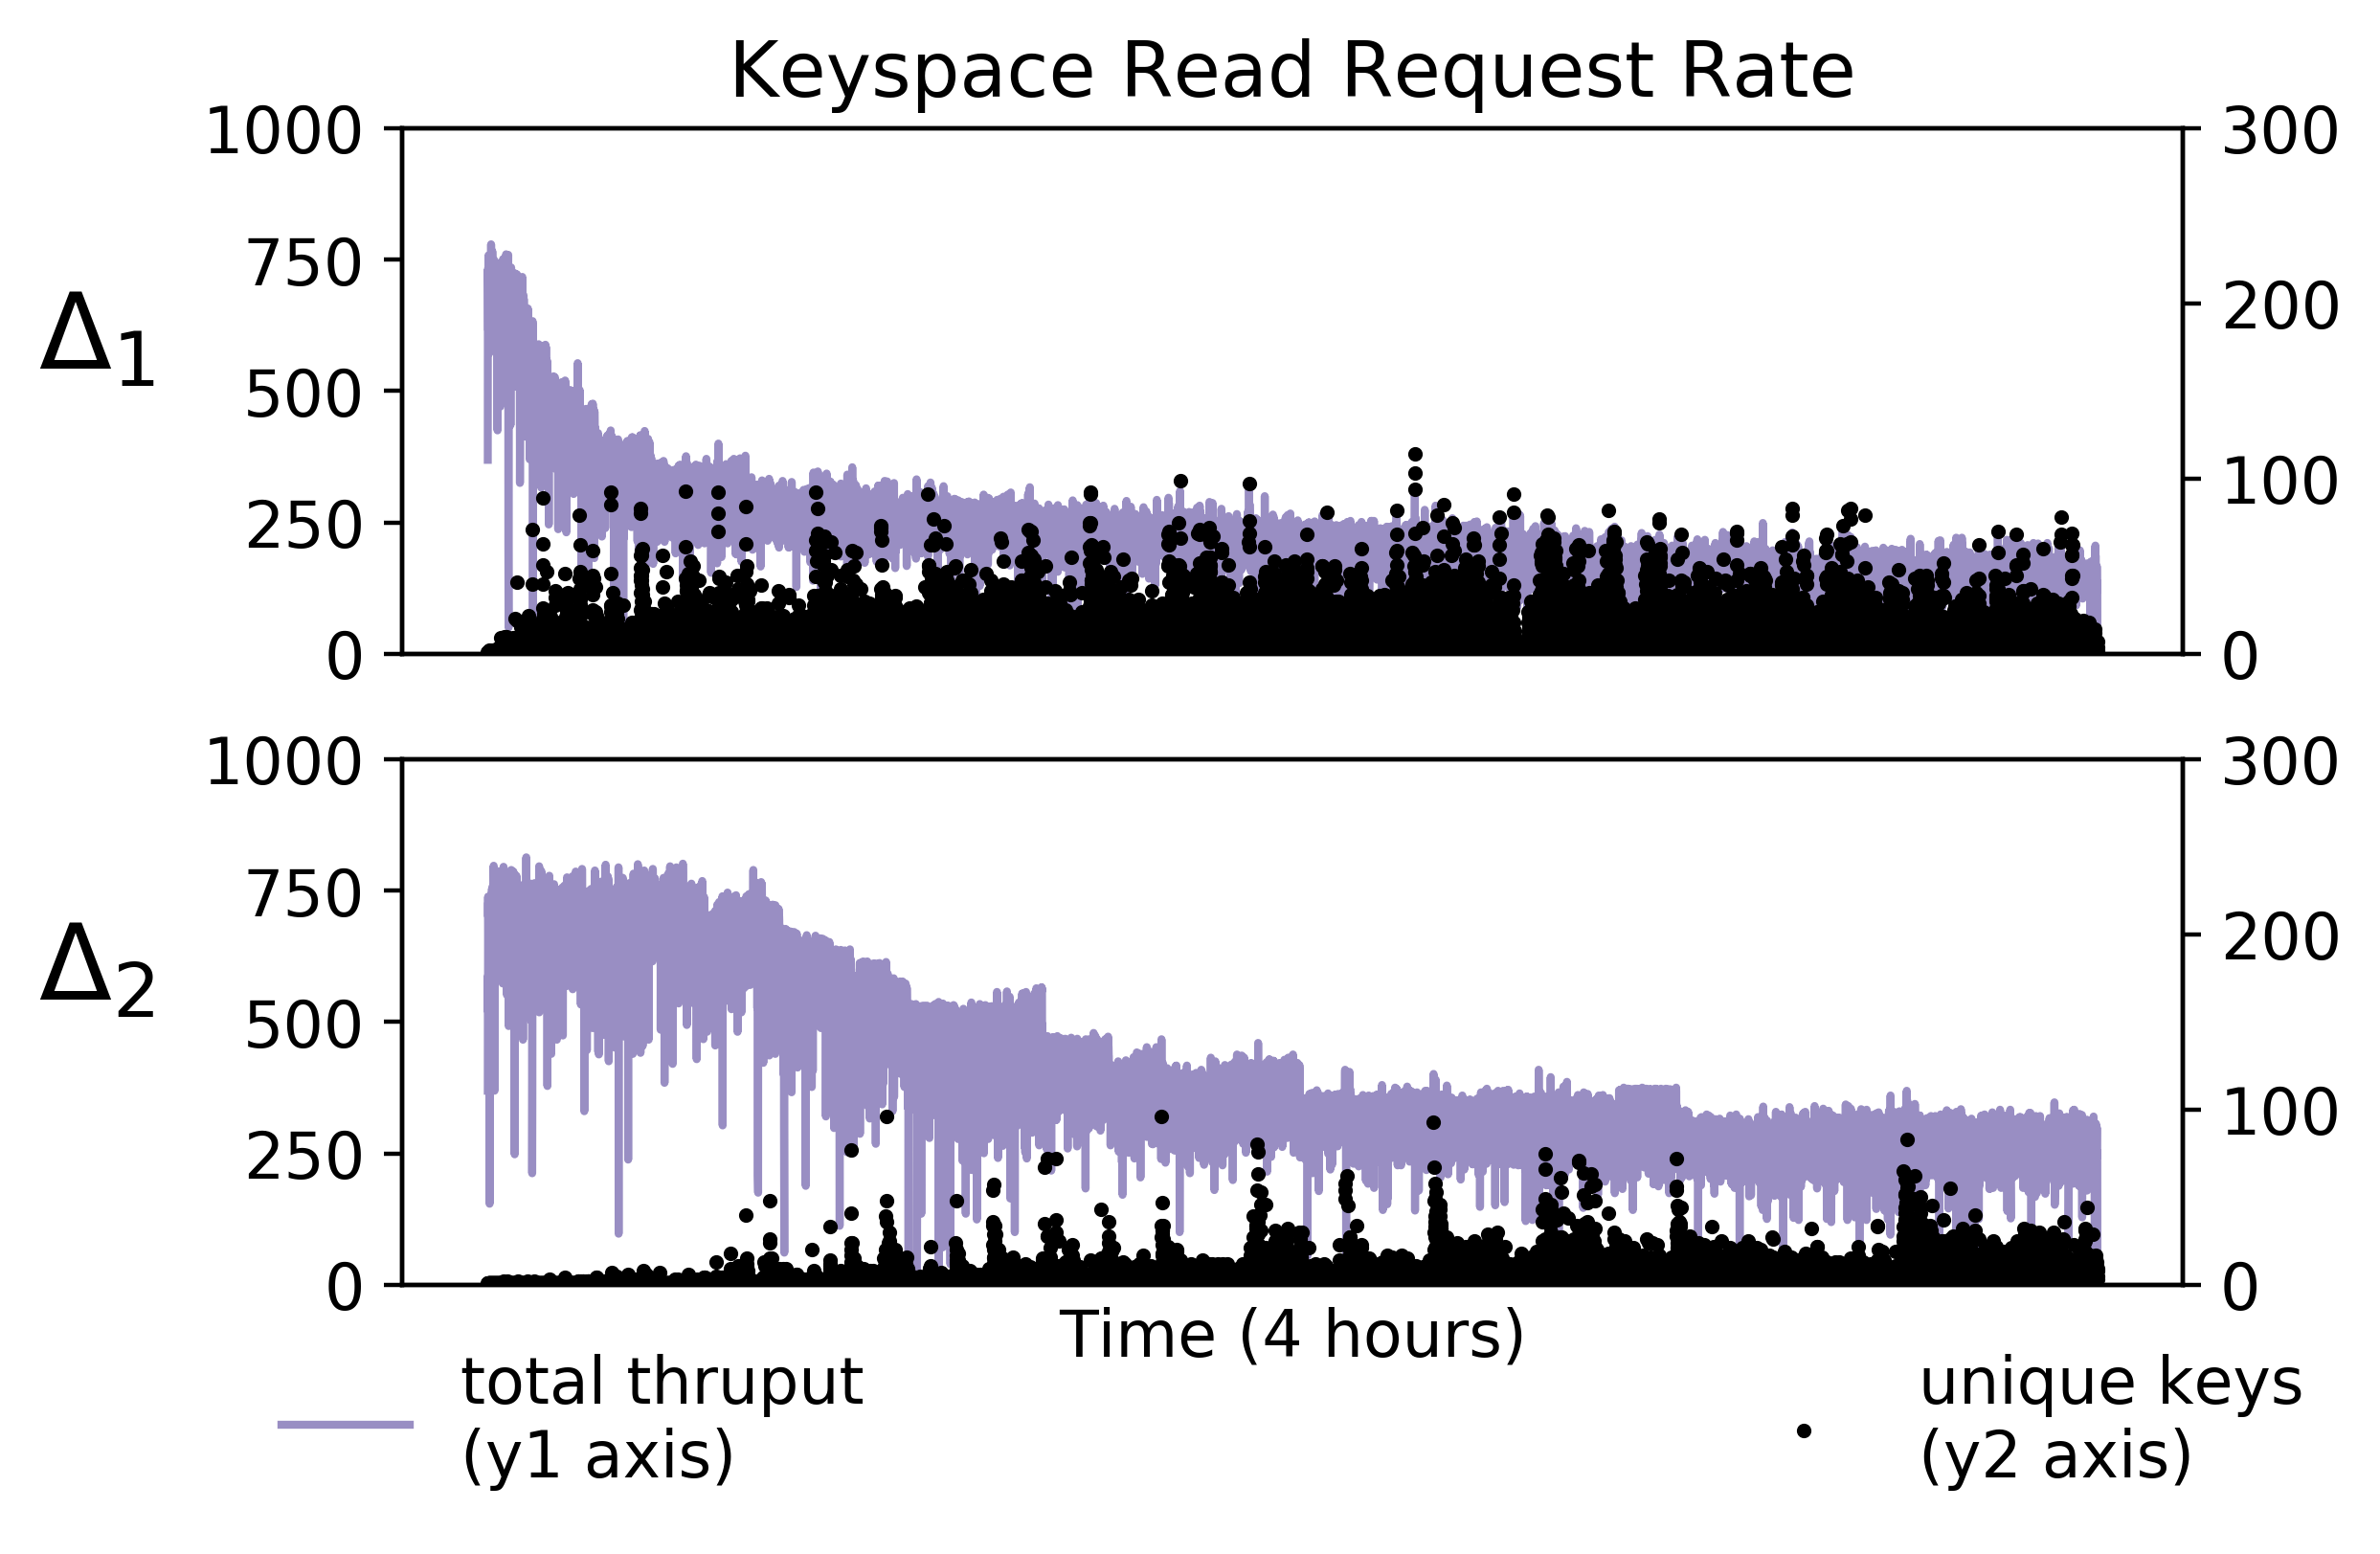
\includegraphics[width=0.5\textwidth]{figures/motivation-regimes.png}\\
  \caption{The keyspace activity for ParSplice using two different growth
rates.  The line shows the rate that EOM minima values are retrieved from the
key-value store (\(y1\) axis) and the points along the bottom show the number
of keys accessed in a 1 second sliding window (\(y2\) axis).
\label{fig:motivation-regimes}}
\end{figure}

In this paper we present a detailed analysis of how the ParSplice application
accesses key-value pairs over the course of a long running simulation across a
variety of initial conditions.  This type of analysis (1) shows the capacity
and resource requirements of a single node and (2) will help inform our load
balancing policies for when we switch to a distributed key-value store back-end
to store EOM minima. We need to know when and how to partition the keyspace: a
smaller cache hurts performance because key-value pairs need to be retrieved
from other nodes while a larger cache has higher memory pressure.

For example, Figure~\ref{fig:motivation-regimes} shows the
cache activity of a ParSplice node and demonstrates that small changes to the
rates at which new atoms enter the simulation (\(\Delta\)) can have a strong
effect on the timing and frequency with which new EOM minima are discovered and
referenced.  The ParSplice caches on each node are trimmed when memory pressure
reaches a threshold but the number of unique keys accessed (black points
along bottom of both graphs) in Figure~\ref{fig:motivation-regimes} suggests
that a small cache of EOM minima should be sufficient. 

% What is Mantle
To explore the effects of different cache management strategies, we link the
Mantle policy engine into ParSplice.  Mantle~\cite{sevilla:sc15-mantle} has
already proven to be a critical control plane for improving file system
metadata load balancing  and in this work we show its usefulness in cache
management for the changing key-value workloads generated by ParSplice.
Developers write policies for ``when" they want data moved, ``where" they want
data moved, and ``how much" of the data to move and the framework executes
these policies whenever a decision needs to be made.  This abstraction helps
developers unfamiliar with the domain quickly reason about, develop, and deploy
new policies that control temporal and spatial locality. We show that Mantle:

\begin{itemize}

  \item decomposes cache management into independent policies that can be
  dynamically changed, making the problem more manageable and facilitating rapid
  development. Changing the policy in use is critical in applications such as
  ParSplice that have alternating stable and chaotic keyspace access patterns
  over the course of a long-running simulation.  

  \item can be used to quickly deploy a variety of cache management strategies,
  ranging from basic algorithms and heuristics to statistical models and machine
  learning.

  \item has useful primitives that, while designed for file system metadata
  load balancing, turn out to also be effective for cache management. This
  finding shows how the policy engine generalizes to different domains and
  enables control of policies by machines instead of administrators.

\end{itemize}

% this gives us many policies that are effective across disciplines
% - reuse: eases burden of writing policies
% - autonomic: lays groundwork for an adaptable policy that mixes/matches policies
% FUTURE WORK

This last contribution is explored in Section~\S\ref{sec:mantle-brains}, where
we try a range of policies from different disciplines; but more importantly, in
Section~\S\ref{sec:relation-to-file-systems}, we conclude that the collection
of policies we designed for ParSplice's cache management are very similar to
the policies in the Ceph file system that are used to load balance metadata,
suggesting that there is potential for automatically adapting and generating
policies dynamically. 

%Manageable: abstracts away complexities of the system (pass around to others,
%use different strategies) 

